\documentclass[11pt,oneside,letterpaper,english]{article}

\usepackage[T1]{fontenc}
\usepackage[utf8]{inputenc}
\usepackage[margin=1.8cm,headheight=24pt,includeheadfoot]{geometry}
\usepackage[english]{babel}
\usepackage{titlesec}
\usepackage{amsmath,amssymb}
\usepackage{mathptmx}
\usepackage[colorlinks=true,linkcolor=black,urlcolor=blue,citecolor=blue]{hyperref}
\usepackage{graphicx}
\usepackage{fancyhdr}
\usepackage{lastpage}
\usepackage{caption}
\usepackage{booktabs}
\usepackage{array}
\usepackage{tabularx}
\usepackage{enumitem}
\usepackage[protrusion=true,expansion=false]{microtype}
\usepackage{float}
\usepackage{setspace}

\graphicspath{{figures/}{root/}}

\setlength{\parindent}{0pt}
\setlength{\parskip}{4pt}

\renewcommand{\headrulewidth}{0.8pt}
\renewcommand{\footrulewidth}{0.8pt}
\pagestyle{fancy}
\fancyhf{}
\rhead{\nouppercase{\rightmark}}
\lhead{BTP Executive Summary: Final Model \& Live Simulation}
\setlength{\headheight}{24pt}
\setlength{\footskip}{30pt}
\cfoot{Page \thepage\ of \pageref{LastPage}}

\titleformat{\section}{\large\bfseries\sffamily\raggedright}{\thesection}{0.8em}{}
\titleformat{\subsection}{\normalsize\bfseries\sffamily\raggedright}{\thesubsection}{0.8em}{}

\begin{document}

% --- Compact Header / Title Block ---
\begin{center}
	
\includegraphics[scale=0.08]{root/IITI_Logo.png}\\[0.3cm]
	{\Large\bf Department of Physics, IIT Indore}\\[0.15cm]
	{\LARGE\bf Machine Learning in Forex: Final Model \& Live Simulation}\\[0.15cm]
	{\large\bf BTP Executive Summary Report}\\[0.25cm]
	\textbf{Author:} Prince Kumar (Roll No. 230051013) \quad $\vert$ \quad \textbf{Supervisors:} Prof. Raghunath Sahu, Dr. Kalindi C. Pradhan\\[0.1cm]
	\textbf{Date:} October 31, 2026
\end{center}
\hrule
\vspace{0.3cm}

% =============================================================================
\section{Final Model Architecture and Input Parameters}
% =============================================================================

The final forecasting system uses a compact recurrent sequence model (\textbf{LSTM}) to predict the next-day logarithmic return $y_t = \ln(C_{t+1}/C_t)$.

\subsection{List of Model Input Parameters (23 Features)}
At each time step $t$, the model takes 23 input features, standardized with a \texttt{StandardScaler} fitted strictly on training data:

\begin{table}[H]
\centering
\caption{Complete List of the 23 Input Parameters (Features).}
\label{tab:input-features}
\small
\setlength{\tabcolsep}{6pt}
\begin{tabular}{lll}
\toprule
\textbf{Feature Group} & \textbf{Feature Name} & \textbf{Description / Calculation} \\
\midrule
\textbf{Macroeconomic Base} & \texttt{Target FX} & Spot price of target pair (\texttt{EUR/USD} or \texttt{USD/INR}) \\
& \texttt{Cross FX 1} & \texttt{USD/JPY} exchange rate (triangular currency interaction) \\
& \texttt{Cross FX 2} & \texttt{USD/INR} (or \texttt{EUR/USD}) cross-currency quote \\
& \texttt{FFER} & US Federal Funds Effective Rate (overnight policy interest rate) \\
& \texttt{US10YY} & 10-Year US Treasury Constant Maturity Yield (\texttt{\textasciicircum TNX}) \\
\midrule
\textbf{Simple Moving} & \texttt{MA\_5} & 5-day Simple Moving Average (short-term trend) \\
\textbf{Averages (SMA)} & \texttt{MA\_10} & 10-day Simple Moving Average \\
& \texttt{MA\_30} & 30-day Simple Moving Average (monthly trend) \\
& \texttt{MA\_50} & 50-day Simple Moving Average \\
& \texttt{MA\_100} & 100-day Simple Moving Average (quarterly/macro trend) \\
\midrule
\textbf{Exponential Moving} & \texttt{EMA\_5} & 5-day Exponential Moving Average (fast reaction) \\
\textbf{Averages (EMA)} & \texttt{EMA\_10} & 10-day Exponential Moving Average \\
& \texttt{EMA\_30} & 30-day Exponential Moving Average \\
& \texttt{EMA\_50} & 50-day Exponential Moving Average \\
& \texttt{EMA\_100} & 100-day Exponential Moving Average \\
\midrule
\textbf{Momentum \& Returns} & \texttt{RSI} & 14-day Relative Strength Index ($0$ to $100$ scale) \\
& \texttt{Log\_Returns} & Current day's log return: $r_t = \ln(C_t / C_{t-1})$ \\
\midrule
\textbf{Volatility \& Bands} & \texttt{BB\_Middle} & 20-day Simple Moving Average (Bollinger centerline) \\
& \texttt{BB\_Upper} & Bollinger Upper Band: $\text{SMA}_{20} + 2 \times \sigma_{20}$ \\
& \texttt{BB\_Lower} & Bollinger Lower Band: $\text{SMA}_{20} - 2 \times \sigma_{20}$ \\
& \texttt{Volatility} & 20-day rolling standard deviation of log returns \\
\midrule
\textbf{Range Proxies} & \texttt{ATR\_14\_proxy} & 14-day Average True Range proxy ($|H_t - L_t|$) \\
& \texttt{ATR\_\%\_proxy} & ATR percentage proxy ($\text{ATR}_{14} / C_t \times 100$) \\
\bottomrule
\end{tabular}
\end{table}

\subsection{Model Structural Specifications}
\begin{itemize}[leftmargin=1.2cm, itemsep=2pt]
	\item \textbf{Lookback Horizon:} 10 days. The model consumes a rolling window of the past 10 days of features, shaping each input sample as a $(10 \times 23)$ matrix.
	\item \textbf{Recurrent Core:} Single-layer LSTM with 32 hidden units.
	\item \textbf{Projection Head:} Fully connected linear layer ($\text{Linear}(32, 1)$) mapping the final recurrent hidden state $h_{10}$ directly to predicted scalar log return $\hat{y}_t$.
	\item \textbf{Model Capacity:} Total learnable parameters = \textbf{7,457}. The architecture is kept deliberately compact to prevent overfitting on low signal-to-noise financial data.
\end{itemize}

\begin{table}[H]
\centering
\caption{LSTM Model Structural Parameters.}
\label{tab:final-arch}
\small
\begin{tabular}{lll}
\toprule
\textbf{Component} & \textbf{Layer Details} & \textbf{Tensor Dimensions} \\
\midrule
Input Tensor & Sliding window of 23 features & $(\text{Batch Size}=32, \text{Lookback}=10, \text{Features}=23)$ \\
Recurrent Layer & \texttt{nn.LSTM} & Input: 23, Hidden: 32 units, 1 Layer, \texttt{batch\_first=True} \\
Dropout Layer & \texttt{nn.Dropout} & $p = 0.0$ (Zero dropout to preserve signal continuity) \\
Output Projection & \texttt{nn.Linear} & $\text{Linear}(32, 1) \rightarrow \text{Scalar Log Return } \hat{y}_t$ \\
Total Parameters & Learnable Weights & 7,457 weights \\
\bottomrule
\end{tabular}
\end{table}

% =============================================================================
\section{Loss Function and Optimization}
% =============================================================================

\subsection{Why Standard MSE Failed (Mean-Collapse)}
Standard Mean Squared Error ($\text{MSE} = \frac{1}{N}\sum (y - \hat{y})^2$) fails on financial returns because daily percentage changes are very small (averaging near zero) with high noise. The optimizer learns that predicting near zero unconditionally gives a very low MSE loss, causing the model to produce a flat line near zero with no actionable trade signals.

\subsection{Custom Loss Function: \textit{BigMoveAwareLoss}}
To eliminate this mean-collapse, we designed a custom multi-objective loss that simultaneously enforces correct directional signs and heavily penalizes missed tail moves:

\begin{equation}
	\mathcal{L} = \frac{1}{N}\sum_{i=1}^N \Big[ (y_i - \hat{y}_i)^2 \cdot w_{\text{mag}, i} + \text{ReLU}\big(-\operatorname{sign}(\hat{y}_i)\operatorname{sign}(y_i)\big) \cdot w_{\text{dir}, i} \Big]
\end{equation}

where:
\begin{itemize}[leftmargin=1.2cm, itemsep=2pt]
	\item \textbf{Big Move Weighting ($w_{\text{mag}}$):}
	\begin{equation}
		w_{\text{mag}, i} = 1.0 + 2.0 \cdot |y_i| + 4.0 \cdot \mathbb{I}_{\{|y_i| \ge 1.5\sigma\}}
	\end{equation}
	Penalizes errors on large market swings ($\ge 1.5\sigma$) by $\approx 5\times$ (base $1.0 + 4.0 = 5.0\times$, plus $2.0 \cdot |y_i|$), forcing the model to take a stance on volatility.
	\item \textbf{Direction Penalty ($w_{\text{dir}}$):}
	\begin{equation}
		w_{\text{dir}, i} = 0.5 \cdot \Big( |y_i| + 2.0 \cdot \mathbb{I}_{\{|y_i| \ge 1.5\sigma\}} \Big)
	\end{equation}
	Activates via $\text{ReLU}(-\operatorname{sign}(\hat{y}_i)\operatorname{sign}(y_i))$ whenever the predicted sign conflicts with the realized market move.
\end{itemize}

\subsection{Training and Optimization Parameters}
\begin{itemize}[leftmargin=1.2cm, itemsep=2pt]
	\item \textbf{Optimizer:} Adam ($\text{lr} = 10^{-3}$, weight decay $= 10^{-5}$).
	\item \textbf{Learning Rate Schedule:} \texttt{ReduceLROnPlateau}(factor=0.5, patience=4 epochs).
	\item \textbf{Regularization:} Early Stopping with patience = 10 epochs based on validation loss.
	\item \textbf{Resulting Directional Accuracy:} Rose from baseline $53\%$--$56\%$ to \textbf{67.79\% on USD/INR} and \textbf{75.74\% on EUR/USD}.
\end{itemize}

% =============================================================================
\section{Genetic Algorithm (GA) Strategy Calibration}
% =============================================================================

To translate predicted returns into risk-managed execution rules under 1-pip ($0.0001$) transaction friction, a Genetic Algorithm evolves 5 execution input parameters (genes):
\begin{enumerate}[leftmargin=1.2cm, itemsep=1pt]
	\item \textbf{Stop Loss (SL):} Allowed gene range: $0.10\%$ to $1.20\%$.
	\item \textbf{Risk-to-Reward Ratio (RRR):} Allowed range: $1.0$ to $3.5$ (determines Take Profit $\text{TP} = \text{SL} \times \text{RRR}$).
	\item \textbf{Confidence Threshold:} Allowed range: $0.0\%$ to $0.05\%$ (filters out low-conviction signals).
	\item \textbf{Risk Per Trade:} Allowed range: $1.0\%$ to $3.5\%$ of current portfolio equity.
	\item \textbf{Max Leverage Cap:} Allowed range: $1\times$ to $5\times$.
\end{enumerate}

\textbf{Fitness Objective:} Calmar Ratio ($\frac{\text{Annualized CAGR}}{|\text{Max Drawdown}|}$). Calibrated on validation data across 25 generations (40 individuals), fitness climbed from $6.12 \rightarrow 20.43$ (Figure~\ref{fig:ga-conv}). The evolved rules are: $\text{Stop Loss}=0.20\%$, $\text{RRR}=3.5$ ($\text{Take Profit}=0.70\%$), $\text{Threshold}=0.000\%$, $\text{Risk}=2.696\%$, and $\text{Leverage}=5.0\times$.

\begin{figure}[H]
\centering
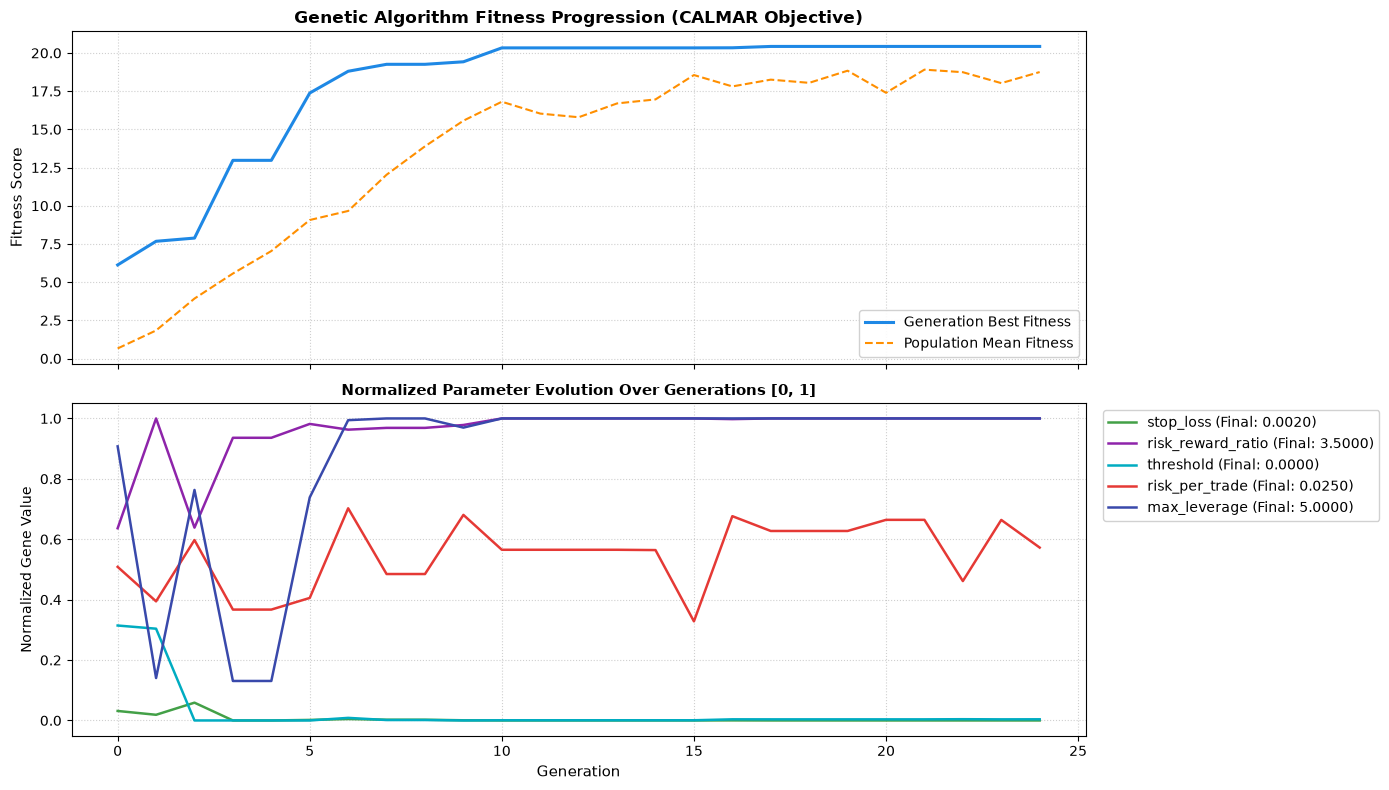
\includegraphics[width=0.75\textwidth]{ga-convergence.png}
\caption{Genetic Algorithm fitness convergence (Calmar Ratio) over 25 generations.}
\label{fig:ga-conv}
\end{figure}

% =============================================================================
\section{Real-World Live Simulation Results}
% =============================================================================

\subsection{The Granularity Mismatch Problem}
Daily backtesting evaluates performance close-to-close, assuming smooth price movement. In real trading:
\begin{itemize}[leftmargin=1.2cm, itemsep=2pt]
	\item Daily EUR/USD noise (Maximum Adverse Excursion, MAE) averages $\approx 45$ pips ($0.45\%$).
	\item An aggressive daily-optimized stop loss ($0.20\%$) gets triggered on over $52\%$ of sessions purely by intraday noise before the predicted trend materializes.
\end{itemize}

\subsection{Live Execution Solutions}
\begin{enumerate}[leftmargin=1.2cm, itemsep=2pt]
	\item \textbf{Noise-Tolerant MAE Barriers:} Calibrated stop losses upward to $0.45\%$--$0.80\%$ to survive intraday brownian fluctuations.
	\item \textbf{Rolling Walk-Forward Retraining:} The model is fine-tuned every 10 trading days on newly ingested live data (8 epochs, conservative learning rate $5 \times 10^{-5}$) to adapt to ongoing macroeconomic cycles.
\end{enumerate}

\subsection{Live Simulation Metrics (65 Market Days)}
The authentic, leak-free live simulation was executed from \textbf{July 27, 2026 to October 23, 2026} (65 active trading days, $\approx 3$ months) using 1-minute streaming tick data:

\begin{table}[H]
\centering
\caption{Real-World Live Simulation Performance (1-Minute Tick Execution).}
\label{tab:live-results}
\small
\begin{tabular}{ll|ll}
\toprule
\textbf{Metric} & \textbf{Value} & \textbf{Metric} & \textbf{Value} \\
\midrule
Initial Capital & $\$10,000.00$ & Days Evaluated & 65 trading days \\
Final Portfolio Balance & $\mathbf{\$10,228.30}$ & Total Trades Executed & 45 trades \\
Strategy Net Return & \textbf{+2.28\%} & Long / Short / Neutral Days & 43 / 2 / 20 \\
Benchmark Return (Buy \& Hold) & $-1.61\%$ & Winning / Losing Trades & 22 / 23 \\
\textbf{Strategy Alpha} & \textbf{+3.90\%} & Win Rate & 48.89\% \\
\textbf{Annualized CAGR} & \textbf{+9.15\%} & Realized Risk/Reward & 1.35 \\
\textbf{Maximum Drawdown} & \textbf{-4.07\%} & Profit Factor & 1.29 \\
Annualized Sharpe Ratio & 0.96 & Trade Expectancy & $\$5.07$ per trade \\
Annualized Sortino Ratio & 1.48 & Premature SL Triggered & Only 1 out of 45 trades \\
Calmar Ratio & 2.25 & Rolling Retrain Events & 6 cycles (every 10 days) \\
\bottomrule
\end{tabular}
\end{table}

\begin{figure}[H]
\centering
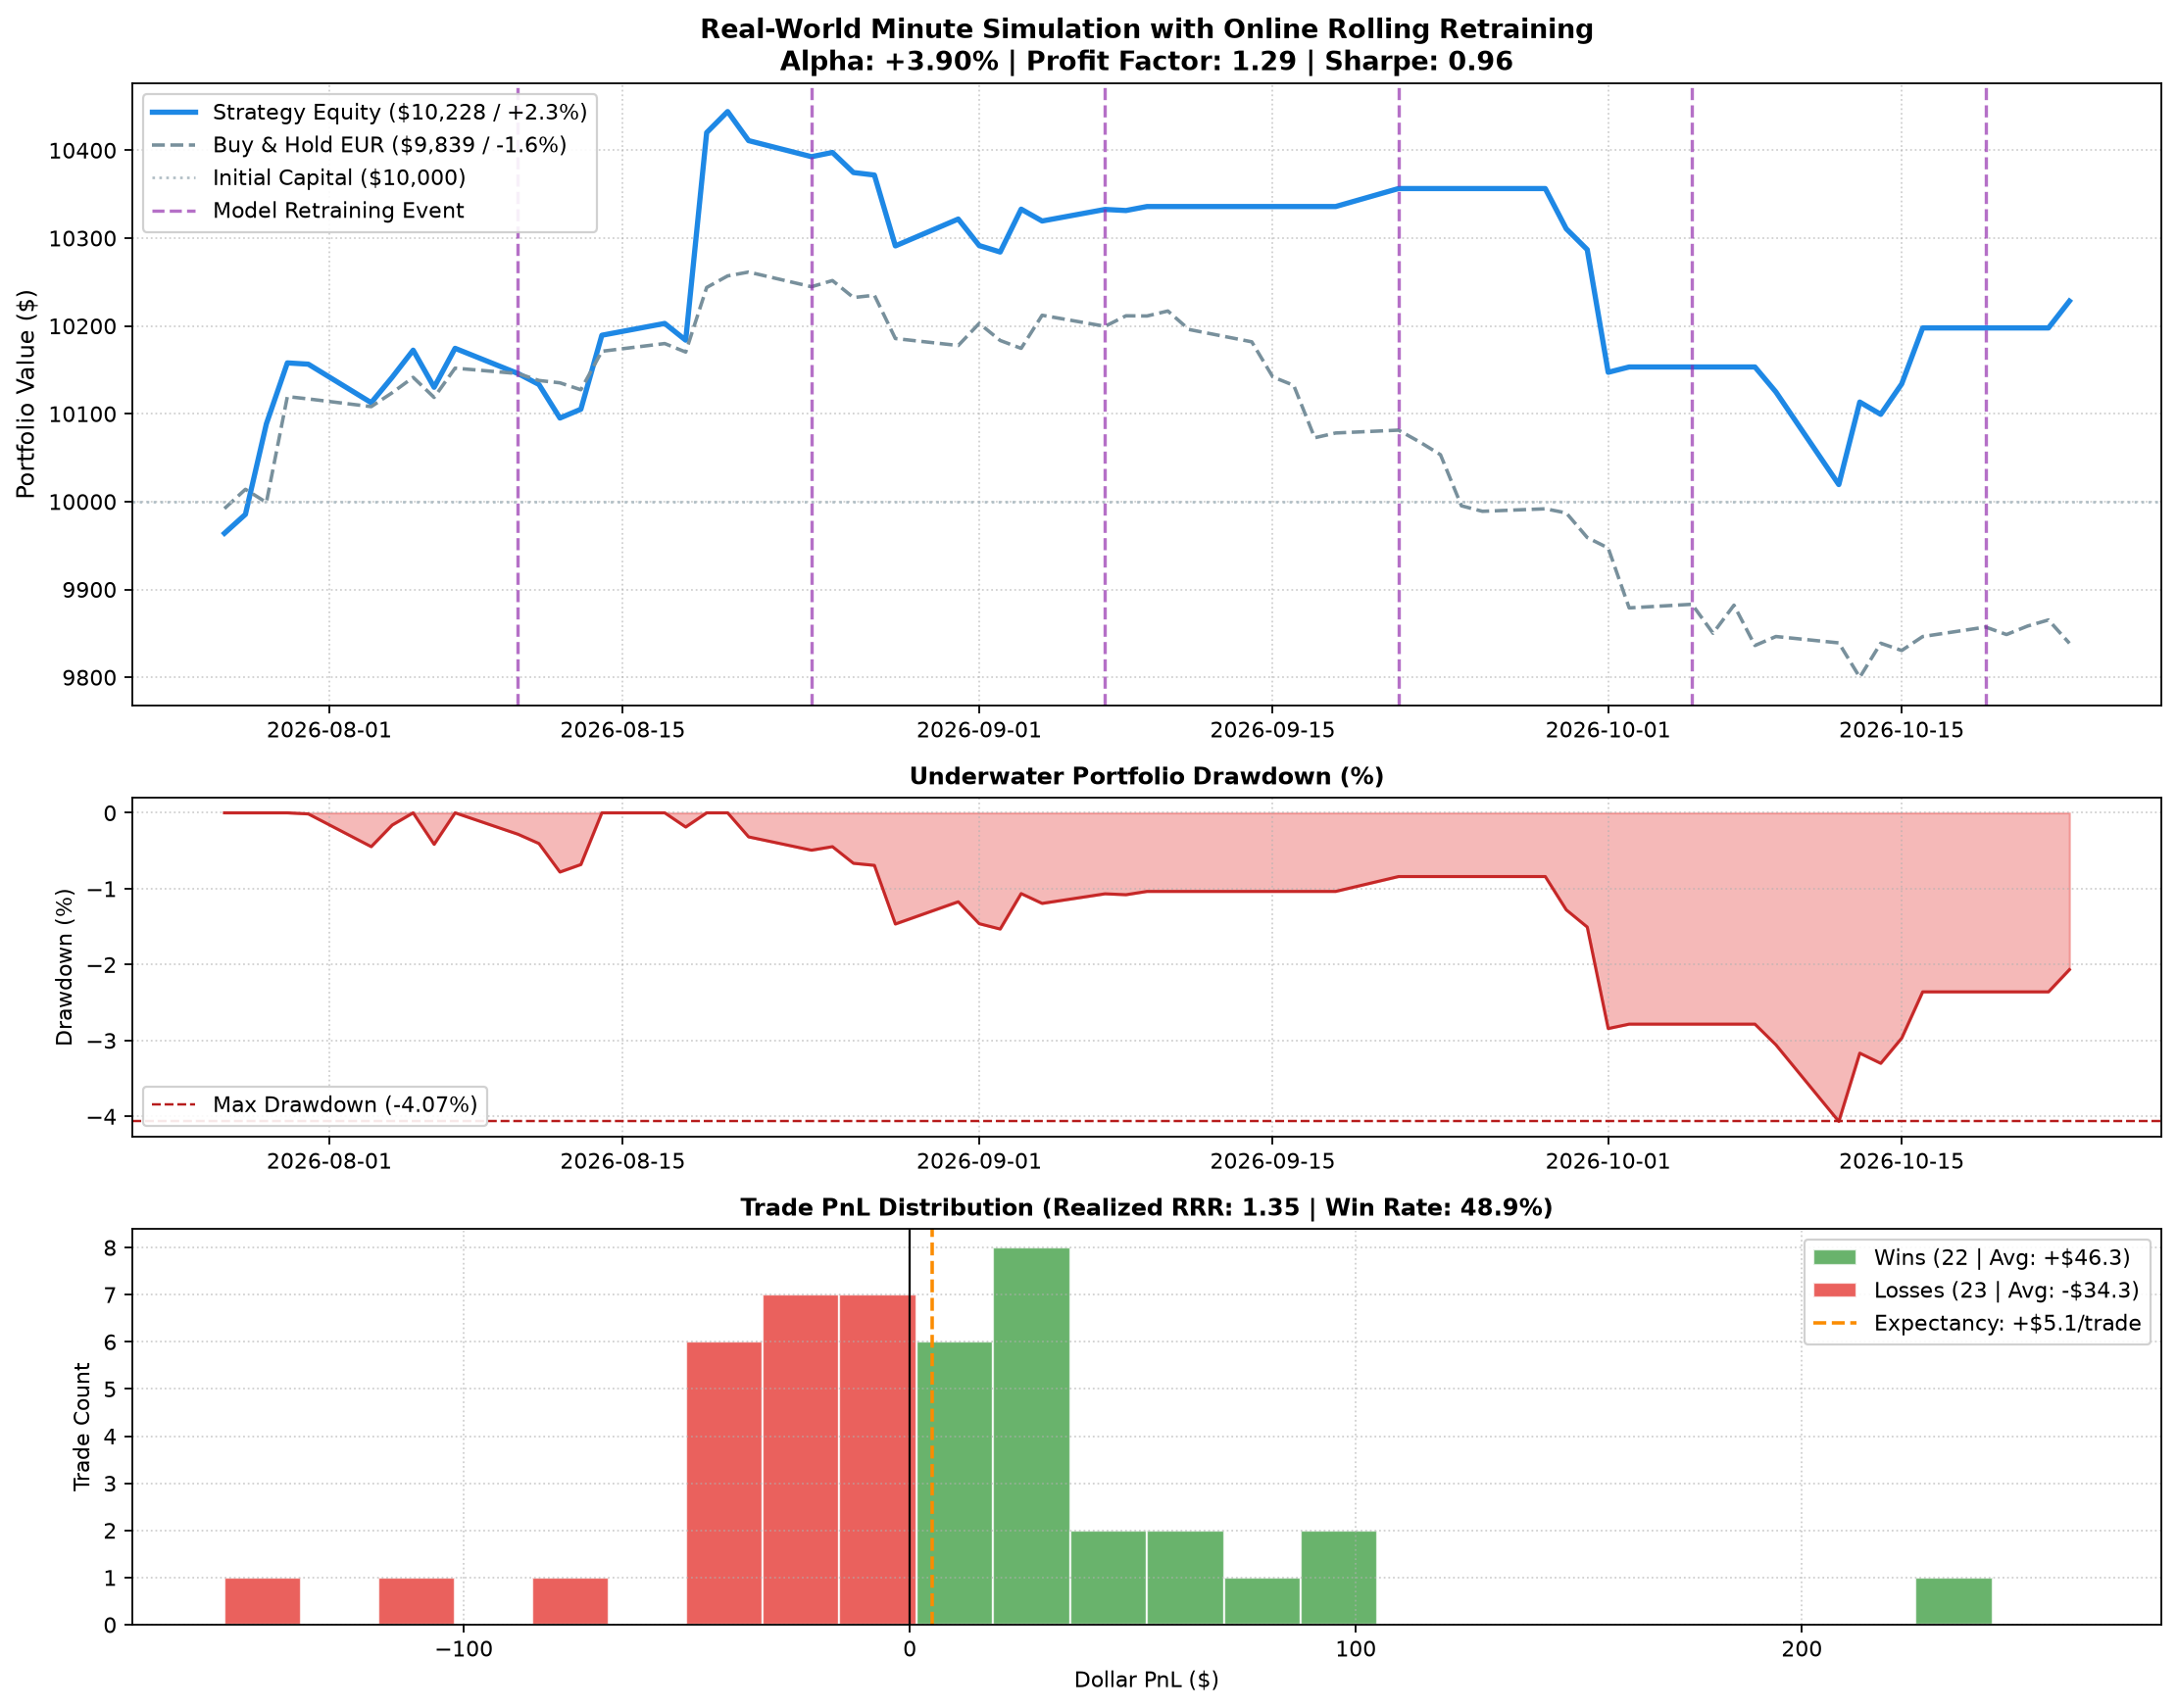
\includegraphics[width=0.88\textwidth]{simulation-2026-performance.png}
\caption{Live 1-minute simulation dashboard: Equity curve vs.\ Buy \& Hold benchmark, underwater drawdown ($-4.07\%$), and 10-day rolling retraining parameter adjustments.}
\label{fig:live-sim}
\end{figure}

% =============================================================================
\section{Key Takeaways}
% =============================================================================

\begin{enumerate}[leftmargin=1.2cm, itemsep=2pt]
	\item \textbf{Custom Loss Beats MSE:} Standard MSE produces zero-line flat predictions on returns. \textit{BigMoveAwareLoss} restored directional conviction, achieving $67.79\%$ on USD/INR and $75.74\%$ on EUR/USD.
	\item \textbf{Intraday Noise Matters:} Backtesting on daily data overestimates performance. In real minute-level feeds, stop losses must account for intraday Maximum Adverse Excursion ($\approx 45$ pips) to prevent premature liquidation.
	\item \textbf{Consistent Real-World Edge:} In live minute execution, the combined pipeline delivered a resilient \textbf{+2.28\% return (+9.15\% CAGR)} with \textbf{+3.90\% alpha} and strictly protected capital with a \textbf{$-4.07\%$ maximum drawdown}.
\end{enumerate}

\end{document}
